\documentclass[11pt]{article}
\input{headers03}

\usepackage{fancyhdr}   
\pagestyle{fancy}      
\lhead{CS 355, FALL 2020}               
\rhead{Name: Christopher Cohen} %%% <-- REPLACE Hemanta K. Maji WITH YOUR NAME HERE

\usepackage[strict]{changepage}  
\newcommand{\nextoddpage}{\checkoddpage\ifoddpage{\ \newpage\ \newpage}\else{\ \newpage}\fi}  


\begin{document}

\title{Homework 3}

\date{}

\maketitle 

\thispagestyle{fancy}  
\pagestyle{fancy}      




\begin{enumerate}
%%%%%%%%%%%%%%%%%%%%%%%%%%%%%%%%%%%%%%%%%%%%%%%%%%
%%%%%%%%%%%% PROBLEM 1 %%%%%%%%%%%%%%%%%%%%%%%%%%%%
%%%%%%%%%%%%%%%%%%%%%%%%%%%%%%%%%%%%%%%%%%%%%%%%%%%
\item {\bfseries Security of encryption schemes (8+8+8 points).} For each of the encryption schemes below, state whether the scheme is secure or not. Justify your answer in each case. 
\begin{enumerate}
    \item The message space is $\cM = \{0,1, \dotsc, 6 \}$. Algorithm $\gen$ chooses a uniform key from the key space $\cK = \{1, \dotsc, 6\}$. The encryption algorithm $\enc_{sk}(m)$ returns $(sk+m) \mod 7$, and the decryption algorithm $\dec_{sk}(m)$ returns $(c-sk) \mod 7$.\newline
    % ANSWER %
    {\bfseries
    One of the properties of an encryption scheme states that a scheme is secure if and only if, $\forall x, y$ distinct, $wt(x,c) = wt(y,c)$: \newline
    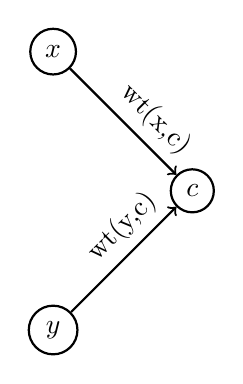
\begin{tikzpicture}[node distance={25mm}, thick, main/.style = {draw, circle}] 
      \node[main] (1) {$x$}; 
      \node[main] (2) [below right of=1] {$c$};
      \node[main] (3) [below left of=2] {$y$};
      \draw[->] (1) -- node[midway, above left, sloped, pos=1] {wt(x,c)} (2);
      \draw[->] (3) -- node[midway, above left, sloped, pos=1] {wt(y,c)} (2);
    \end{tikzpicture} \newline

    I will prove this by contradiction - we only need one example where this doesn't hold true. Let's look at the messages $0$ and $1$. Their graphs for a couple of encodings are shown below. The secret key that witnesses the message's encoding to the given ciphertext is labeled on the connecting line.

    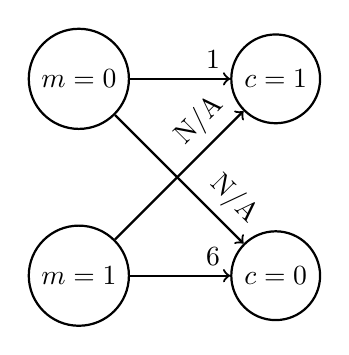
\begin{tikzpicture}[node distance={25mm}, thick, main/.style = {draw, circle}] 
      \node[main] (1) {$m=0$}; 
      \node[main] (2) [right of=1] {$c=1$};

      \node[main] (3) [below of=1] {$m=1$};
      \node[main] (4) [right of=3] {$c=0$};


      \draw[->] (1) -- node[midway, above left, sloped, pos=1] {1} (2);
      \draw[->] (3) -- node[midway, above left, sloped, pos=1] {6} (4);
      \draw[->] (1) -- node[midway, above left, sloped, pos=1] {N/A} (4);
      \draw[->] (3) -- node[midway, above left, sloped, pos=1] {N/A} (2);
    \end{tikzpicture} \newline

    Clearly, we can see that the weights are uneven. Here is the rundown: \newline
    $wt(0,0) = 0$, $wt(0,1) = 1 \newline
    wt(1,0) = 1$, $wt(1,1) = 0$
    
    Since we stated earlier that, for a scheme to be secure, $wt(x,c)=wt(y,c)$. In this example, we can see that $wt(0,0)=0$ and $wt(1,0)=1$, which contradicts our earlier statement. Therefore, we can conclude that this scheme is insecure.
    }
    %%%%%%%%%%
    \newpage
    \item The message space is $\cM = \{0,1, \dotsc, 6 \}$. Algorithm $\gen$ chooses a uniform key from the key space $\cK = \{0,1, \dotsc, 7\}$. The encryption algorithm $\enc_{sk}(m)$ returns $(sk+m) \mod 7$, and the decryption algorithm $\dec_{sk}(m)$ returns $(c-sk) \mod 7$.
    % ANSWER %
    {\bfseries
    \newline
    \newline
    Using the same logic as the last part, this scheme is secure. Reiterating, a scheme is secure if and only if $\forall x,y$ distinct, $wt(x,c) = wt(y,c)$. One way that this can be accomplished is if every possible message maps to every possible ciphertext exactly once (aka, all weights are 1). For proof, there is an illustration of the first 2 messages below. Due to the fact that the scheme is uniform (i.e., the encryption method doesn't change for each message), the pattern shown in the sample size below will continue as shown here. \newline


    \begin{table}[htb]
      \centering
      \caption{As you can see, every element$\mod7$ appears once, so all of the weights are the same.}
      \begin{tabular}{|c|c|c|c|c|}
        \hline
        \bfseries{M} & \bfseries{SK} & \bfseries{C}  \\ \hline
       0 & 1 & 1  \\ \hline
       0 & 2 & 2  \\ \hline
       0 & 3 & 3  \\ \hline
       0 & 4 & 4  \\ \hline
       0 & 5 & 5  \\ \hline
       0 & 6 & 6  \\ \hline
       0 & 7 & 0  \\ \hline
       1 & 1 & 2  \\ \hline
       1 & 2 & 3  \\ \hline
       1 & 3 & 4  \\ \hline
       1 & 4 & 5  \\ \hline
       1 & 5 & 6  \\ \hline
       1 & 6 & 0  \\ \hline
       1 & 7 & 1  \\ \hline
      \end{tabular}
    \end{table}
    }
    %%%%%%%%%%
    \newpage
    \item The message space is $\cM=\{1,3,5,\dots,2019,2021\}$. Algorithm $\gen$ chooses a uniform key from the key space $\cK = \{0,2,4,6, \dotsc,2020\}$. The encryption algorithm $\enc_{sk}(m)$ returns $(sk+m) \mod 2022$, and the decryption algorithm $\dec_{sk}(m)$ returns $(c-sk) \mod 2022$. \newline
    % ANSWER %
    {\bfseries
    \newline
    \newline

    Again, this part will use the same logic as the previous two parts. In order for a private-key encryption scheme to be secure, for $\forall x,y$ distinct, $wt(x,c) = wt(y,c)$. Much like the previous part, one way that this can be accomplished is if every possible message maps to every possible ciphertext exactly once (aka, all weights are 1). You will see that, because of the circular pattern of the modulus operator, this scheme accomplishes this. Obviously, not all possible outcomes are shown here, but much like part (b), the pattern will continue.
    
    \begin{table}[htb]
      \centering
      \caption{As you can see, if this were to be fully listed out, every element$\mod2022$ would appear once, so all of the weights are the same.}
      \begin{tabular}{|c|c|c|c|c|}
        \hline
        \bfseries{M} & \bfseries{SK} & \bfseries{C}  \\ \hline
       1 & 0 & 1  \\ \hline
       1 & 2 & 3  \\ \hline
       1 & 4 & 5  \\ \hline
       1 & 6 & 7  \\ \hline
       3 & 2020 & 1  \\ \hline
       3 & 0 & 3  \\ \hline
       3 & 2 & 5  \\ \hline
       3 & 4 & 7  \\ \hline
       5 & 2018  & 1  \\ \hline
       5 & 2020  & 3  \\ \hline
       5 & 0 & 5  \\ \hline
       5 & 2 & 7  \\ \hline
       7 & 2016  & 1  \\ \hline
       7 & 2018  & 3  \\ \hline
       7 & 2020  & 5  \\ \hline
       7 & 0 & 7  \\ \hline
      \end{tabular}
    \end{table}
    }
    %%%%%%%%%%
     
\end{enumerate}

\newpage

%%%%%%%%%%%%%%%%%%%%%%%%%%%%%%%%%%%%%%%%%%%%%%%%%%
%%%%%%%%%%%% PROBLEM 2 %%%%%%%%%%%%%%%%%%%%%%%%%%%%
%%%%%%%%%%%%%%%%%%%%%%%%%%%%%%%%%%%%%%%%%%%%%%%%%%%
\item {\bfseries Equivalent definition of Perfect Secrecy (15 points).} 
In the lecture we defined the perfect security for any private-key encryption scheme $(\pred{Gen},\pred{Enc},\pred{Dec})$ as follows. 
For any message $m$, cipher-text $c$, and a priori probability distribution $\M$ over the set of messages, we have: 
$$ \probX{ \M=m \vert \C=c } = \probX{\M=m}$$
Show that the above definition is \underline{equivalent} to the following alternative definition.  
For all messages $m,m'$, cipher-text $c$, and a priori probability distribution $\M$ over the set of messages, we have: 
$$ \probX{\C=c \vert \M=m} = \probX{\C = c \vert \M=m'},$$

{\footnotesize Remarks: 
(1) Proving equivalence means that you have to show that the first definition implies the second definition. 
And, the second definition also implies the first definition.

(2) Additionally, in this problem, for simplicity, assume that in the probability expressions no ``division by error'' occurs.}

    % ANSWER %
    {\bfseries
    First, I will prove that $ \probX{\C=c \vert \M=m} = \probX{\C = c \vert \M=m'}$. Using Baye's rule, we can do the following: \newline 
    $\probX{\C=c \vert \M=m} = \probX{\C=c \vert \M=m'} \newline
    \frac{\probX{\C=c , \M=m}}{\probX{\M=m}} = \frac{\probX{\C=c , \M=m'}}{\probX{\M=m'}} \newline
    \frac{\probX{\C=c}*\probX{\M=m}}{\probX{\M=m}} = \frac{\probX{\C=c}*\probX{\M=m'}}{\probX{\M=m'}}$ \newline
    Remember that, since every message $m$ is unique, the probability that $\M$ is some value is equally likely for all messages (aka, $\probX{\P=m}$ is constant). Therefore, we can cancel those statements in the numerators and denominators, and we get: \newline
    $\probX{\C=c} = \probX{\C=c}$ \newline
    Therefore, the two statements are equivalent. \newline

    Next, we need to prove that the first and second definitions are equal. We know that, for perfect security, $\forall m, m'$ distinct, $wt(m,c) = wt(m',c)$. For simplicity's sake, let's say that $wt = 1$. This means that each message $m$ uniquely maps to a ciphertext $c$, witnessed by a unique secret key $sk$, as illustrated below:

    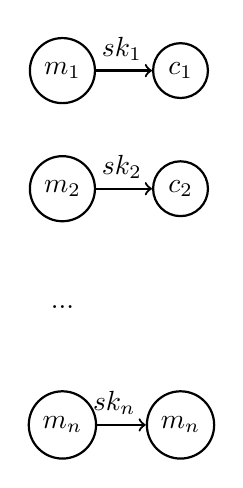
\begin{tikzpicture}[node distance={15mm}, thick, main/.style = {draw, circle}] 
      \node[main] (1) {$m_1$}; 
      \node[main] (2) [right of=1] {$c_1$};

      \node[main] (3) [below of=1] {$m_2$};
      \node[main] (4) [right of=3] {$c_2$};

      \node[] (5) [below of=3] {...};

      \node[main] (6) [below of=5] {$m_n$};
      \node[main] (7) [right of=6] {$m_n$};


      \draw[->] (1) -- node[midway, above left, sloped, pos=1] {$sk_1$} (2);
      \draw[->] (3) -- node[midway, above left, sloped, pos=1] {$sk_2$} (4);
      \draw[->] (6) -- node[midway, above left, sloped, pos=1] {$sk_n$} (7);
    \end{tikzpicture} \newline

    Since all $m$ and $c$ must be in the same message space, and each element in $\M$ and $\C$ are unique, $\probX{\M=m} = \probX{\C=c}$. Therefore, since the first definition evaluates to $\probX{\M=m}$, and the second definition evaluates to $\probX{\C=c}$, we can conclude that the two definitions are equivalent.
    }
    %%%%%%%%%%
     \newpage


%%%%%%%%%%%%%%%%%%%%%%%%%%%%%%%%%%%%%%%%%%%%%%%%%%
%%%%%%%%%%%% PROBLEM 3 %%%%%%%%%%%%%%%%%%%%%%%%%%%%
%%%%%%%%%%%%%%%%%%%%%%%%%%%%%%%%%%%%%%%%%%%%%%%%%%%
\item {\bfseries Defining Perfect Security from Ciphertexts (15 points).} An upstart in the field of cryptography has proposed a new definition for perfect security of private-key encryption schemes. 
According to this new definition, a private-key encryption scheme $(\pred{Gen},\pred{Enc},\pred{Dec})$ is perfectly secure, if, for all a priori distribution $\M$ over the message space, and any two cipher-texts $c$ and $c'$, we have the following identity. 
$$\probX{\C=c} = \probX{\C=c'}$$
Show that the definition in the class does \ul{not} imply this new definition.  

{\footnotesize Remark. 
You need to construct a private-key encryption scheme that is secure according to the definition we learned in the class. 
However, this scheme does not satisfy the new definition.}
    % ANSWER %
    {\bfseries
    \newline
    \newline
    In class, we learned that a private key encryption scheme is secure if $\probX{\M=m \vert \C=c} = \probX{\M=m}$. In order to refute this, we need to construct a scheme in which possible ciphertexts are unevenly weighted. However, we still need to satisfy the definition learned in class. If we expand the definition from class using Baye's theorem, we get the following: \newline

    $\probX{\M=m \vert \C=c} = \frac{\probX{\M=m}*\probX{\C=c}}{\probX{\C=c}} = \probX{\M=m}$ \newline

    This simply means that, in order for a scheme to fit this definition, the ciphertext $c$ must not depend on the input $m$. Imagine a private-key encryption scheme similar to one-time pad, except that when encrypting, there is a $\frac23$ probability that a $1$ will be appended to the resulting encrypted message, and a $\frac13$ probability that a $0$ will be appended to the resulting encrypted message. This means that the resulting ciphertext will NOT depend on the input message $m$.

    Therefore, we can say that this scheme is completely secure based on the definition given in class ($\probX{\M=m \vert \C=c} = \probX{\M=m}$). However, we know that a ciphertext $c$ with the last digit $1$ is twice as likely as a ciphertext $c$ with the last digit $0$, so $\probX{\C=c} \neq \probX{\C=c'}$.
    }
    %%%%%%%%%%
     \newpage
     

%%%%%%%%%%%%%%%%%%%%%%%%%%%%%%%%%%%%%%%%%%%%%%%%%%
%%%%%%%%%%%% PROBLEM 4 %%%%%%%%%%%%%%%%%%%%%%%%%%%%
%%%%%%%%%%%%%%%%%%%%%%%%%%%%%%%%%%%%%%%%%%%%%%%%%%%
\item {\bfseries One-time Pad for 4-Alphabet Words (8+8 points).} 
  We interpret alphabets $\mathtt a,\mathtt b,\dotsc,\mathtt z$ as integers $0,1,\dotsc,25$, respectively. 
  We will work over the group $(\bbZ^4_{26},+)$, where $+$ is coordinate-wise integer sum $\mod 26$. 
  For example, $\mathtt{abcx} + \mathtt{aczd} = \mathtt{a d b a}$. 
  
  Now, consider the one-time pad encryption scheme over the group $(\bbZ^4_{26},+)$. 
  \begin{enumerate}
  \item What is the probability that the encryption of the message $\mathtt{kiwi}$ is the cipher text $\mathtt{kiwi}$? \newline
    % ANSWER %
    {\bfseries
    \newline
    \newline
      In order for the encryption of $\mathtt{kiwi}$ to be $\mathtt{kiwi}$, the secret key would have to be $\mathtt{aaaa}$, since the letter $\mathtt{a}$ doesn't change the value of anything (its value is 0). Since every letter has an equal $\frac1{26}$ chance of being chosen, and there are 4 letters, the probability of this is $\frac{1}{26^4}$.
    }
    %%%%%%%%%%
     \vspace{0.3\textheight}
  \item What is the probability that the encryption of the message $\mathtt{kiwi}$ is the cipher text $\mathtt{lime}$? \newline 
    % ANSWER %
    {\bfseries
    \newline
    \newline
      In order for the encryption of $\mathtt{kiwi}$ to be $\mathtt{lime}$, the secret key would have to be $\mathtt{bapv}$. Since every letter has an equal $\frac1{26}$ chance of being chosen, and there are 4 letters, the probability of this is $\frac{1}{26^4}$.
      }
    %%%%%%%%%%
     \newpage
  \end{enumerate}  

%%%%%%%%%%%%%%%%%%%%%%%%%%%%%%%%%%%%%%%%%%%%%%%%%%
%%%%%%%%%%%% PROBLEM 5 %%%%%%%%%%%%%%%%%%%%%%%%%%%%
%%%%%%%%%%%%%%%%%%%%%%%%%%%%%%%%%%%%%%%%%%%%%%%%%%%


\item {\bfseries Lagrange Interpolation(7+7+6 points).} 
We want to derive a part of the Chinese Remainder Theorem using principles of Lagrange Interpolation. Our goal is the following 
\begin{boxedalgo}
Suppose $p$ and $q$ are two distinct primes. Suppose $a\in \{0,\ldots,p-1\}$ and $b\in \{0,\ldots,q-1 \}$. We want to find a natural number $x$ such that 
\begin{align*}
    x \pmod p =a\ \text{and}\ x\pmod q=b 
\end{align*}
\end{boxedalgo}
We shall proceed towards this objective incrementally (similar to the approach of Lagrange interpolation). 
\begin{enumerate}
    \item Find a natural number $x_p$ satisfying $x_p \pmod p = 1$, and $x_p \pmod q =0$. \newline 
    % ANSWER %
    {\bfseries
    \newline
    \newline
    Since $x_p\mod q = 0$, $x_p$ must be a multiple of $q$, such that $x_p=nq$. \newline
    We also know that $x_p\mod p = 1$, so $x_p=np+1$. \newline
    If we set these equations equal, we find the solution for $n$: \newline

    $nq=np+1 \newline
    nq-np=1 \newline
    n(q-p)=1 \newline
    n=\frac{1}{q-p} \newline$

    Plugging that into the previous equations, we get the solution for $x_p$: \newline
    $x_p = np+1 = nq \newline$

    $x_p = \frac{p}{q-p} + 1 = \frac{q}{q-p} \newline$
    }
    %%%%%%%%%%
     \newpage
    \item Find a natural number $x_q$ satisfying $x_q \pmod p = 0$ and $x_q \pmod q =1$. \newline 
    % ANSWER %
    {\bfseries
    \newline
    \newline
    Since $x_q\mod p = 0$, $x_q$ must be a multiple of $p$, such that $x_p=np$. \newline
    We also know that $x_q\mod q = 1$, so $x_q=nq+1$. \newline
    If we set these equations equal, we find the solution for $n$: \newline

    $np=nq+1 \newline
    np-nq=1 \newline
    n(p-q)=1 \newline
    n=\frac{1}{p-q} \newline$

    Plugging that into the previous equations, we get the solution for $x_q$: \newline
    $x_q = nq+1 = np \newline$

    $x_q = \frac{q}{p-q} + 1 = \frac{p}{p-q} \newline$
    }
    %%%%%%%%%%
     \newpage
    \item Find a natural number $x$ satisfying $x \pmod p = a$ and $x \pmod q =b$. \newline 
    % ANSWER %
    {\bfseries
    \newline
    \newline
    From the start, we know that $x=np+a$ and $x=nq+b$, simply by the definition of the$\mod$ operator and the equations given to us. Setting these two equations equal gives us the solution for $n$: \newline
    $np+a=nq+b \newline
    np-nq=b-a \newline
    n(p-q)=b-a \newline
    n=\frac{b-a}{p-q} \newline
    $

    Plugging that into the previous equations, we get the solution for $x$: \newline
    $x=np+a=nq+b \newline$

    $x=\frac{p(b-a)}{p-q}+a = \frac{q(b-a)}{p-q}+b \newline$
    }
    %%%%%%%%%%
     \newpage
\end{enumerate}
 
%%%%%%%%%%%%%%%%%%%%%%%%%%%%%%%%%%%%%%%%%%%%%%%%%%
%%%%%%%%%%%% PROBLEM 6 %%%%%%%%%%%%%%%%%%%%%%%%%%%%
%%%%%%%%%%%%%%%%%%%%%%%%%%%%%%%%%%%%%%%%%%%%%%%%%%%

\item {\bfseries An Illustrative Execution of Shamir's Secret Sharing Scheme (6+10+9 points).} 
  We shall work over the field $(\bbZ_7,+,\times)$. 
  We are interested in sharing a secret among 6 parties such that any 4 parties can reconstruct the secret, but no subset of 3 parties gain any additional information about the secret. 
  
  Suppose the secret is $s=3$. 
  The random polynomial of degree $<4$ that is chosen during the secret sharing steps is $p(X) = X^3+ 2X + 3$. 
  \begin{enumerate}
  \item What are the respective secret shares of parties 1, 2, 3, 4, 5, and 6? \newline 
    % ANSWER %
    {\bfseries
    \newline
    \newline
      Party 1 - $p(X) = 1^3 + 2(1) + 3 = 6$

      Party 2 - $p(X) = 2^3 + 2(2) + 3 = 15$

      Party 3 - $p(X) = 3^3 + 2(3) + 3 = 36$

      Party 4 - $p(X) = 4^3 + 2(4) + 3 = 75$

      Party 5 - $p(X) = 5^3 + 2(5) + 3 = 138$

      Party 6 - $p(X) = 6^3 + 2(6) + 3 = 231$
    }
    %%%%%%%%%%
     \newpage
  \item Suppose parties 1, 2, 5, and 6 are interested in reconstructing the secret. 
    Run Lagrange Interpolation algorithm as explained in the class. 
    
    ({\footnotesize {\em 
      Remark:} 
      It is essential to show the step-wise reconstruction procedure to score full points. 
      In particular, you need to write down the polynomials $p_1(X)$, $p_2(X)$, $p_3(X)$, and $p_4(X)$.% 
    })\newline 
    % ANSWER %
    {\bfseries
      \newline
      \newline

      Recall the secret shares for parties 1, 2, 5, and 6 are the following: \newline
      Party 1 - 6  --> $(x_1,y_1) = (1,6)$ \newline
      Party 2 - 15  --> $(x_2,y_2) = (2,15)$ \newline
      Party 5 - 138  --> $(x_3,y_3) = (5,138)$ \newline
      Party 6 - 231  --> $(x_4,y_4) = (6,231)$ \newline

      By Lagrange, \newline
      $p_1(X) = y_1 * \frac{(x-x_2)(x-x_3)(x-x_4)}{(x_1-x_2)(x_1-x_3)(x_1-x_4)} = 6 * \frac{(x-2)(x-5)(x-6)}{(1-2)(1-5)(1-6)} = \frac{-3x^3}{10} + \frac{39x^2}{10} - \frac{78}{5} + 18$ \newline
      \newline
      $p_2(X) = y_2 * \frac{(x-x_1)(x-x_3)(x-x_4)}{(x_2-x_1)(x_2-x_3)(x_2-x_4)} = 15 * \frac{(x-1)(x-5)(x-6)}{(2-1)(2-5)(2-6)} = \frac{5x^3}{4} - 15x^2 + \frac{205x}{4} - \frac{75}{2}$ \newline
      \newline
      $p_3(X) = y_3 * \frac{(x-x_1)(x-x_2)(x-x_4)}{(x_3-x_1)(x_3-x_2)(x_3-x_4)} = 138 * \frac{(x-1)(x-2)(x-6)}{(5-1)(5-2)(5-6)} = -\frac{23x^3}{2} + \frac{207x^2}{2} - 230x + 138$ \newline
      \newline
      $p_4(X) = y_4 * \frac{(x-x_1)(x-x_2)(x-x_3)}{(x_4-x_1)(x_4-x_2)(x_4-x_3)} = 231 * \frac{(x-1)(x-2)(x-5)}{(6-1)(6-2)(6-5)} = \frac{231x^3}{20} - \frac{462x^2}{5} + \frac{3927x}{20} - \frac{231}{2}$ \newline
      \newline

      We know that, to solve the equation, all we need is the following formula:
      $p(X) = \sum p_i(X)$ \newline

      $p(X)=p_1(X) + p_2(X) + p_3(X) + p_4(X)$ \newline

      $p(X)=(\frac{-3x^3}{10} + \frac{39x^2}{10} - \frac{78}{5} + 18) + (\frac{5x^3}{4} - 15x^2 + \frac{205x}{4} - \frac{75}{2}) + (-\frac{23x^3}{2} + \frac{207x^2}{2} - 230x + 138) + (\frac{231x^3}{20} - \frac{462x^2}{5} + \frac{3927x}{20} - \frac{231}{2})$ \newline

      $p(X)=x^3 + 0x^2 + 2x + 3$ \newline
      $p(X)=x^3 + 2x + 3$ \newline

      Which is the original polynomial.

    }
    %%%%%%%%%%
     \newpage
  \item Suppose parties 1, 2, and 5 get together. 
    Let $q_{\widetilde s}(X)$ be the polynomial that is consistent with their shares and the point $(0,\widetilde s)$, for each $\widetilde s\in \bbZ_p$. 
    Write down the polynomials $q_0(X)$, $q_1(X)$, $\dotsc$, $q_6(X)$.  \newline 
    % ANSWER %
    {\bfseries
      Party 1 - 6  --> $(x_1,y_1) = (1,6)$ \newline
      Party 2 - 15  --> $(x_2,y_2) = (2,15)$ \newline
      Party 5 - 138  --> $(x_3,y_3) = (5,138)$ \newline

      $q_0(X)$ is consistent with the shares of parties 1, 2, 5, and the point (0,0). \newline
      $q_0(X) = \frac{13x^3}{10}-\frac{12x^2}{5}+\frac{71x}{10}$ \newline

      $q_1(X)$ is consistent with the shares of parties 1, 2, 5, and the point (0,1). \newline
      $q_1(X) = \frac{6x^3}{5}-\frac{8x^2}{5}+\frac{27x}{5}+1$ \newline

      $q_2(X)$ is consistent with the shares of parties 1, 2, 5, and the point (0,2). \newline
      $q_2(X) = \frac{11x^3}{10}-\frac{4x^2}{5}+\frac{37x}{10}+2$ \newline

      $q_3(X)$ is consistent with the shares of parties 1, 2, 5, and the point (0,3). \newline
      $q_3(X) = x^3+2x+3$ \newline

      $q_4(X)$ is consistent with the shares of parties 1, 2, 5, and the point (0,4). \newline
      $q_4(X) = \frac{9x^3}{10}+\frac{4x^2}{5}+\frac{3x}{10}+4$ \newline

      $q_5(X)$ is consistent with the shares of parties 1, 2, 5, and the point (0,5). \newline
      $q_5(X) = \frac{4x^3}{5}+\frac{8x^2}{5}-\frac{7x}{5}+5$ \newline

      $q_6(X)$ is consistent with the shares of parties 1, 2, 5, and the point (0,6). \newline
      $q_6(X) = \frac{7x^3}{10}+\frac{12^2}{5}-\frac{31x}{10}+6$ \newline
    }
    %%%%%%%%%%
     \newpage
  \end{enumerate}     
     
     

%%%%%%%%%%%%%%%%%%%%%%%%%%%%%%%%%%%%%%%%%%%%%%%%%%
%%%%%%%%%%%% PROBLEM 7 %%%%%%%%%%%%%%%%%%%%%%%%%%%%
%%%%%%%%%%%%%%%%%%%%%%%%%%%%%%%%%%%%%%%%%%%%%%%%%%%   
\item {\bfseries A bit of Counting (8+8+9 points).} 
  In this problem, we will do a bit of counting related to polynomials that pass through a given set of points in the plane. 
  We already did this counting (slightly informally) in the class. 
  Writing the solution for this problem shall make the solution's intuition more concrete. 
  
  We are working over the field $(\bbZ_p,+,\times)$, where $p$ is a prime number. 
  Let $\cP_t$ be the set of all polynomials in the indeterminate $X$ with degree $<t$ and coefficients in $\bbZ_p$. 
  
  \begin{enumerate}
  \item Let $(x_1,y_1)$, $(x_2,y_2)$, $\dotsc$, and $(x_t,y_t)$ be $t$ points in the plane $\bbZ_p^2$. 
    We have that $x_i \neq x_j$ for all $i\neq j$, that is, the first coordinates of the points are all distinct. 
    
    Prove that there exists a {\em unique polynomial} in $\cP_t$ that passes through these $t$ points. 
    
    ({\footnotesize
      Hint: 
        Use Lagrange Interpolation and Schwartz--Zippel Lemma. 
    }%
    )\newline 
    % ANSWER %
    {\bfseries
    \newline
    \newline
      I will prove this by contradiction. So, let's assume that there is NOT a unique polynomial (aka, there is more than one polynomial that passes through all of the points). That means that $\exists p(X), q(X)$ such that $p(x_i)=y_i$ and $q(x_i)=y_i$. \newline

      If we have a polynomial $r(X)$ that is the difference between $p(X)$ and $q(X)$ ($r(X) = p(X) - q(X)$), we can assume the following: \newline
      \begin{enumerate}
        \item $r(X) \neq 0$, since subtracting two distinct polynomials won't equal 0. \newline
        \item By Lagrange, we know that $r(X) = \sum_{i} p(x_i) - q(x_i)$, so $r(x_i) = p(x_i)-q(x_i)$. $p(x_i)=q(x_i)=y_i$, so $r(x_i)=y_i-y_i=0$. \newline
        \item If $r(x_i)=0$, we can conclude that $x_i$ is a root, and since $r(x)$ is the summation of all $r(x_i)$, we can conclude that $x_1, x_2, x_3, \dotsi, x_t$ are ALL roots of $r(X)$. \newline
        \item The degree of $r(X)$ is guaranteed to be $< t$, since both $p(X)$ and $q(X)$ have degree $< t$. \newline
      \end{enumerate}

      By the Schwartz-Zippel Lemma, a non-zero polynomail of degree $t$ has, at most, $t$ roots. Bullet point iv says that the degree $r(X)$ is guaranteed to be $< t$, so that means the maximum amount of roots for $r(X)$ can have is $<t$. However, bullet point iii says that we have $t$ roots, which is not $<t$, which means that our assumption does not hold. Therefore, by contradiction, there must be a unique polynomial that passes through the points $(x_1,y_1)$, $(x_2,y_2)$, $\dotsc$, and $(x_t,y_t)$.
    }
    %%%%%%%%%%
     \newpage
  \item Let $(x_1,y_1)$, $(x_2,y_2)$, $\dotsc$, and $(x_{t-1},y_{t-1})$ be $(t-1)$ points in the plane $\bbZ_p^2$.
    We have that $x_i \neq x_j$ for all $i\neq j$, that is, the first coordinates of the points are all distinct.
    
    Prove that there are $p$ polynomials in $\cP_t$ that pass through these $(t-1)$ points. \newline 
    % ANSWER %
    {\bfseries
    \newline
    \newline
      In the previous problem, we knew there was a unique polynomial because of the fact that we had too many roots ($\geq t$) to satisfy  our statement. In this case, we have $<t$ roots, so there need not exist a unique polynomial. The question is, how many are there? \newline

      Again, from the previous problem, we know that, for $t$ points, there exists a unique polynomial with $t$ roots that passes through them. Say that, for this problem, we have a similar polynomial with $t$ roots. We only have $t-1$ roots that need to be satisfied, so there is $1$ root that can be whatever we want. Any root in $\bbZ_p$ will work! Since there are $p$ elements in $\bbZ_p$, there are $p$ polynomials in $\cP_t$ that pass through these $(t-1)$ points.
    }
    %%%%%%%%%%
     \newpage
  \item Let  $(x_1,y_1)$, $(x_2,y_2)$, $\dotsc$, and $(x_k,y_k)$ be $k$ points in the plane $\bbZ_p^2$, where $k\leq t$. 
    We have that $x_i \neq x_j$ for all $i\neq j$, that is, the first coordinates of the points are all distinct.
    
    Prove that there are $p^{t-k}$ polynomials in $\cP_t$ that pass through these $k$ points. \newline 
    % ANSWER %
    {\bfseries
    \newline
    \newline
      We know from part (a) that $t$ points gives us 1 unique polynomial that passes through all $t$ points. This follows the equation here. Since $k=t$, $p^{t-k}=p^0=1$ polynomial. \newline

      We also know from part (b) that $t-1$ points gives us $p$ unique polynomials that pass through all $(t-1)$ points. This also follows the equation. Since $k=t-1$, $p^{t-k}=p^{t-(t-1)}=p^1=p$. \newline

      Using the same logic as part (b), we know that if there are $t$ points, there exists a unique polynomial with $t$ roots that passes through all $t$ points. If you only have $(t-1)$ roots to satisfy, there is 1 root that can be whatever we want, making a total of $p$ possible polynomials. For every fewer point that we need to satisfy, we gain a power of $p$ possibilities. This means that if we only need to satisfy $(t-2)$ points, we have $p*p=p^2$ possibilities, $(t-3)$ roots gives $p*p*p=p^3$ possibilities, $(t-x)$ roots gives $p^x$ possibilities, and so on. This clearly proves that there are $p^{t-k}$ polynomials in $\cP_t$ that pass through a given $k$ points.
    }
    %%%%%%%%%%
     \newpage
  \end{enumerate} 

\newpage
     

\end{enumerate}
%%%%%%%%%%%%%%%%%%%%%%%%%%%%%%%%%%%%%%%%%%%%%%%%%%
%%%%%%%%%%%% PLEASE LIST COLLABORATORS BELOW  %%%%%
%%%%%%%%%%%%%%%%%%%%%%%%%%%%%%%%%%%%%%%%%%%%%%%%%%%
{\bfseries Collaborators: N/A} \newline 
% ENTER THEIR NAMES HERE  

\end{document}
